\section{Pianificazione}
Lo sviluppo del progetto è suddiviso nelle seguenti fasi:
    \begin{itemize}
        \item  RTB
        \item PB
    \end{itemize}
    \subsection{RTB}
    Nel periodo dal 04/11/2024 al 17/01/2025 verranno prodotti i seguenti documenti:
        \begin{itemize}
            \item "Norme di progetto"
            \item "Piano di progetto"
            \item "Analisi dei requisiti"
            \item "Piano di qualifica"
            \item "Glossario"
        \end{itemize}
    Inoltre verrà realizzato il Proof of Concept, per valutare la fattibilità tecnologica del progetto.
        \subsubsection{Sprint 1 (dal 11/11/2024 al 22/11/2024)}
        In questo periodo verrà definito il way of working, documentato nelle
        \textit{"Norme di progetto"}. Per quanto riguarda la gestione di progetto, verranno 
        pianificate le attività, stilato un preventivo e analizzati i rischi che potrebbero
        incidere sullo svolgimento del progetto. Infine si comincerà a redigere il 
        \textit{"Glossario"}, fondamentale per garantire una chiara comprensione e comunicazione all'
        interno del team e con il proponente.
        \\
        \begin{figure}[h!]
            \centering
            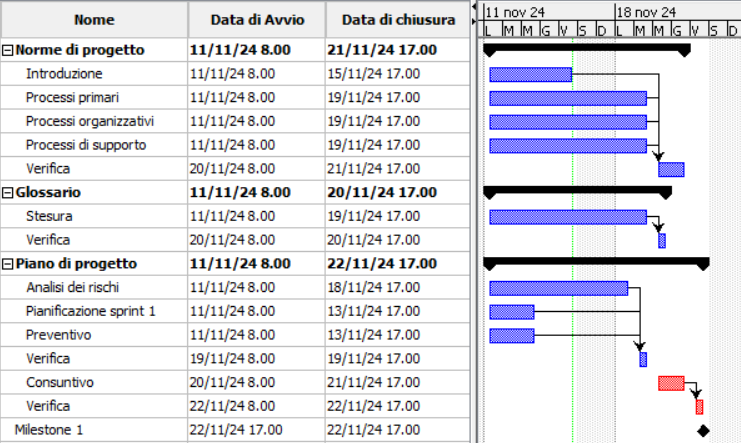
\includegraphics[scale = 0.85]{template/images/gantt1.png}
            \caption{Diagramma di Gantt sprint 1}
            \label{fig:3.1} % Etichetta per il riferimento
        \end{figure}

        \subsubsection{Sprint 2 (dal 25/11/2024 al 06/12/2024)}
        Durante questo secondo sprint, ci dedicheremo alla raccolta e all'analisi dei requisiti, identificando i 
        casi d'uso. Questi saranno documentati nel file \textit{"Analisi dei requisiti"} per garantire una visione 
        chiara degli obiettivi del progetto. Continueremo inoltre l'espansione del \textit{"Glossario"}, già 
        avviato durante lo sprint 1.  Procederemo con l'aggiornamento delle \textit{"Norme di Progetto"} tramite modifiche e miglioramenti per assicurare una gestione ottimale delle attività e delle risorse. Infine, con priorità minore, inizieremo la stesura del \textit{"Piano di Qualifica"}, necessario per definire le metriche e le modalità di 
        verifica della qualità del prodotto.

        
        \begin{figure}[h!]
            \centering
            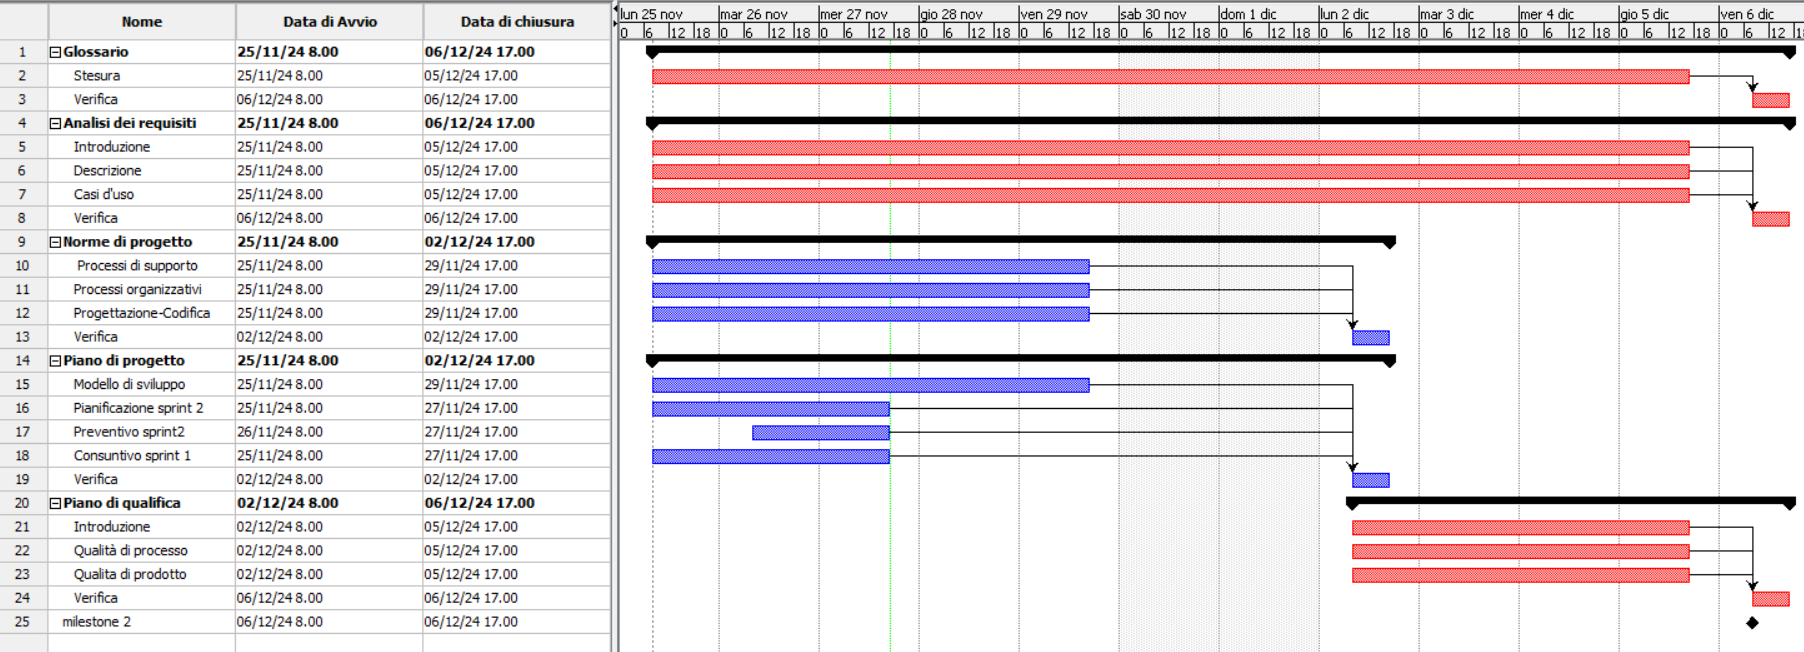
\includegraphics[scale = 0.3]{template/images/gantt2.png}
            \caption{Diagramma di Gantt sprint 2}
            \label{fig:3.2} % Etichetta per il riferimento
        \end{figure}
 
